%% ============================================================
%% 分片 09：原文第 4 节「Compactification And The Geometry Of Hitchin's Moduli Space」（原文 glshort.tex 起于第 2325 行）
%% 由 tools/harvmac2tex.py 从 arXiv 源码（hep-th/0604151v3）自动生成。
%% 只译英文散文；公式、编号、\label、\cite 一律不改。
%% ============================================================

\subsection{$\M_H$ As A Hyper-Kahler Quotient}

\label{sec:mhhyper}

For us the fact of central importance is that $\M_H$ can be
regarded as a hyper-Kahler quotient and therefore is a
hyper-Kahler manifold. Our first goal is to describe how this
comes about.

We consider a problem in gauge theory on a Riemann surface $C$,
the fields being a gauge field $ A$ and a one-form $\phi$ that
takes values in the adjoint representation.  (These arise by
restricting to $C$ the fields $A,\phi$ that appeared in section
第~\ref{sec:tqftfour}~节\ in constructing the twisted gauge theory on a general
four-manifold $M$.)  We think of the space of all fields $A,\phi$
as an infinite-dimensional affine space $\EUW$.  We write $\delta$
for the exterior derivative on $\EUW$ (to denote this as $d$ would
invite confusion with the exterior derivative on $C$; hopefully,
there will be no confusion with the use of the symbol $\delta_S$
in section 第~\ref{sec:tqftfour}~节\ to denote supersymmetric variation).

We define a flat metric on $\EUW$ by % 式 (4.2)
\setcounter{equation}{1}
\begin{equation}\label{eq:igob}
ds^2=-{1\over
4\pi}\int_C|d^2z|\,\Tr\left(\delta A_z\otimes \delta A_{\bar
z}+\delta A_{\bar z}\otimes \delta A_z +\delta \phi_z\otimes
\delta \phi_{\bar z}+\delta \phi_{\bar z}\otimes \delta
\phi_z\right).
\end{equation}
 Here for a local complex coordinate $z$ on $C$, we
write $A=dz\,A_z+d\bar z A_{\bar z}$, $\phi = dz\,\phi_z+d\bar
z\,\phi_{\bar z}$, and $|d^2z|$ is the measure corresponding to
the $(1,1)$-form $i dz\wedge d\bar z$.  This metric on $\EUW$, in
which $\EUW$ is an infinite-dimensional Euclidean space, is
determined by the complex structure on $C$ (and does not depend on
the local coordinate $z$ that we used in writing it).

We want to extend this flat metric on $\EUW$ to a flat
hyper-Kahler structure.  To do this, we introduce three complex
structures $I,J,$ and $K$ on $\EUW$ obeying certain axioms.  They
will all be translation-invariant on the affine space $\EUW$, so
they can be defined by (constant) linear transformations of the
space of one-forms. Any linear transformation of square $-1$ will
define a complex structure; integrability is automatic.

\begin{figure}[htbp]
\centering
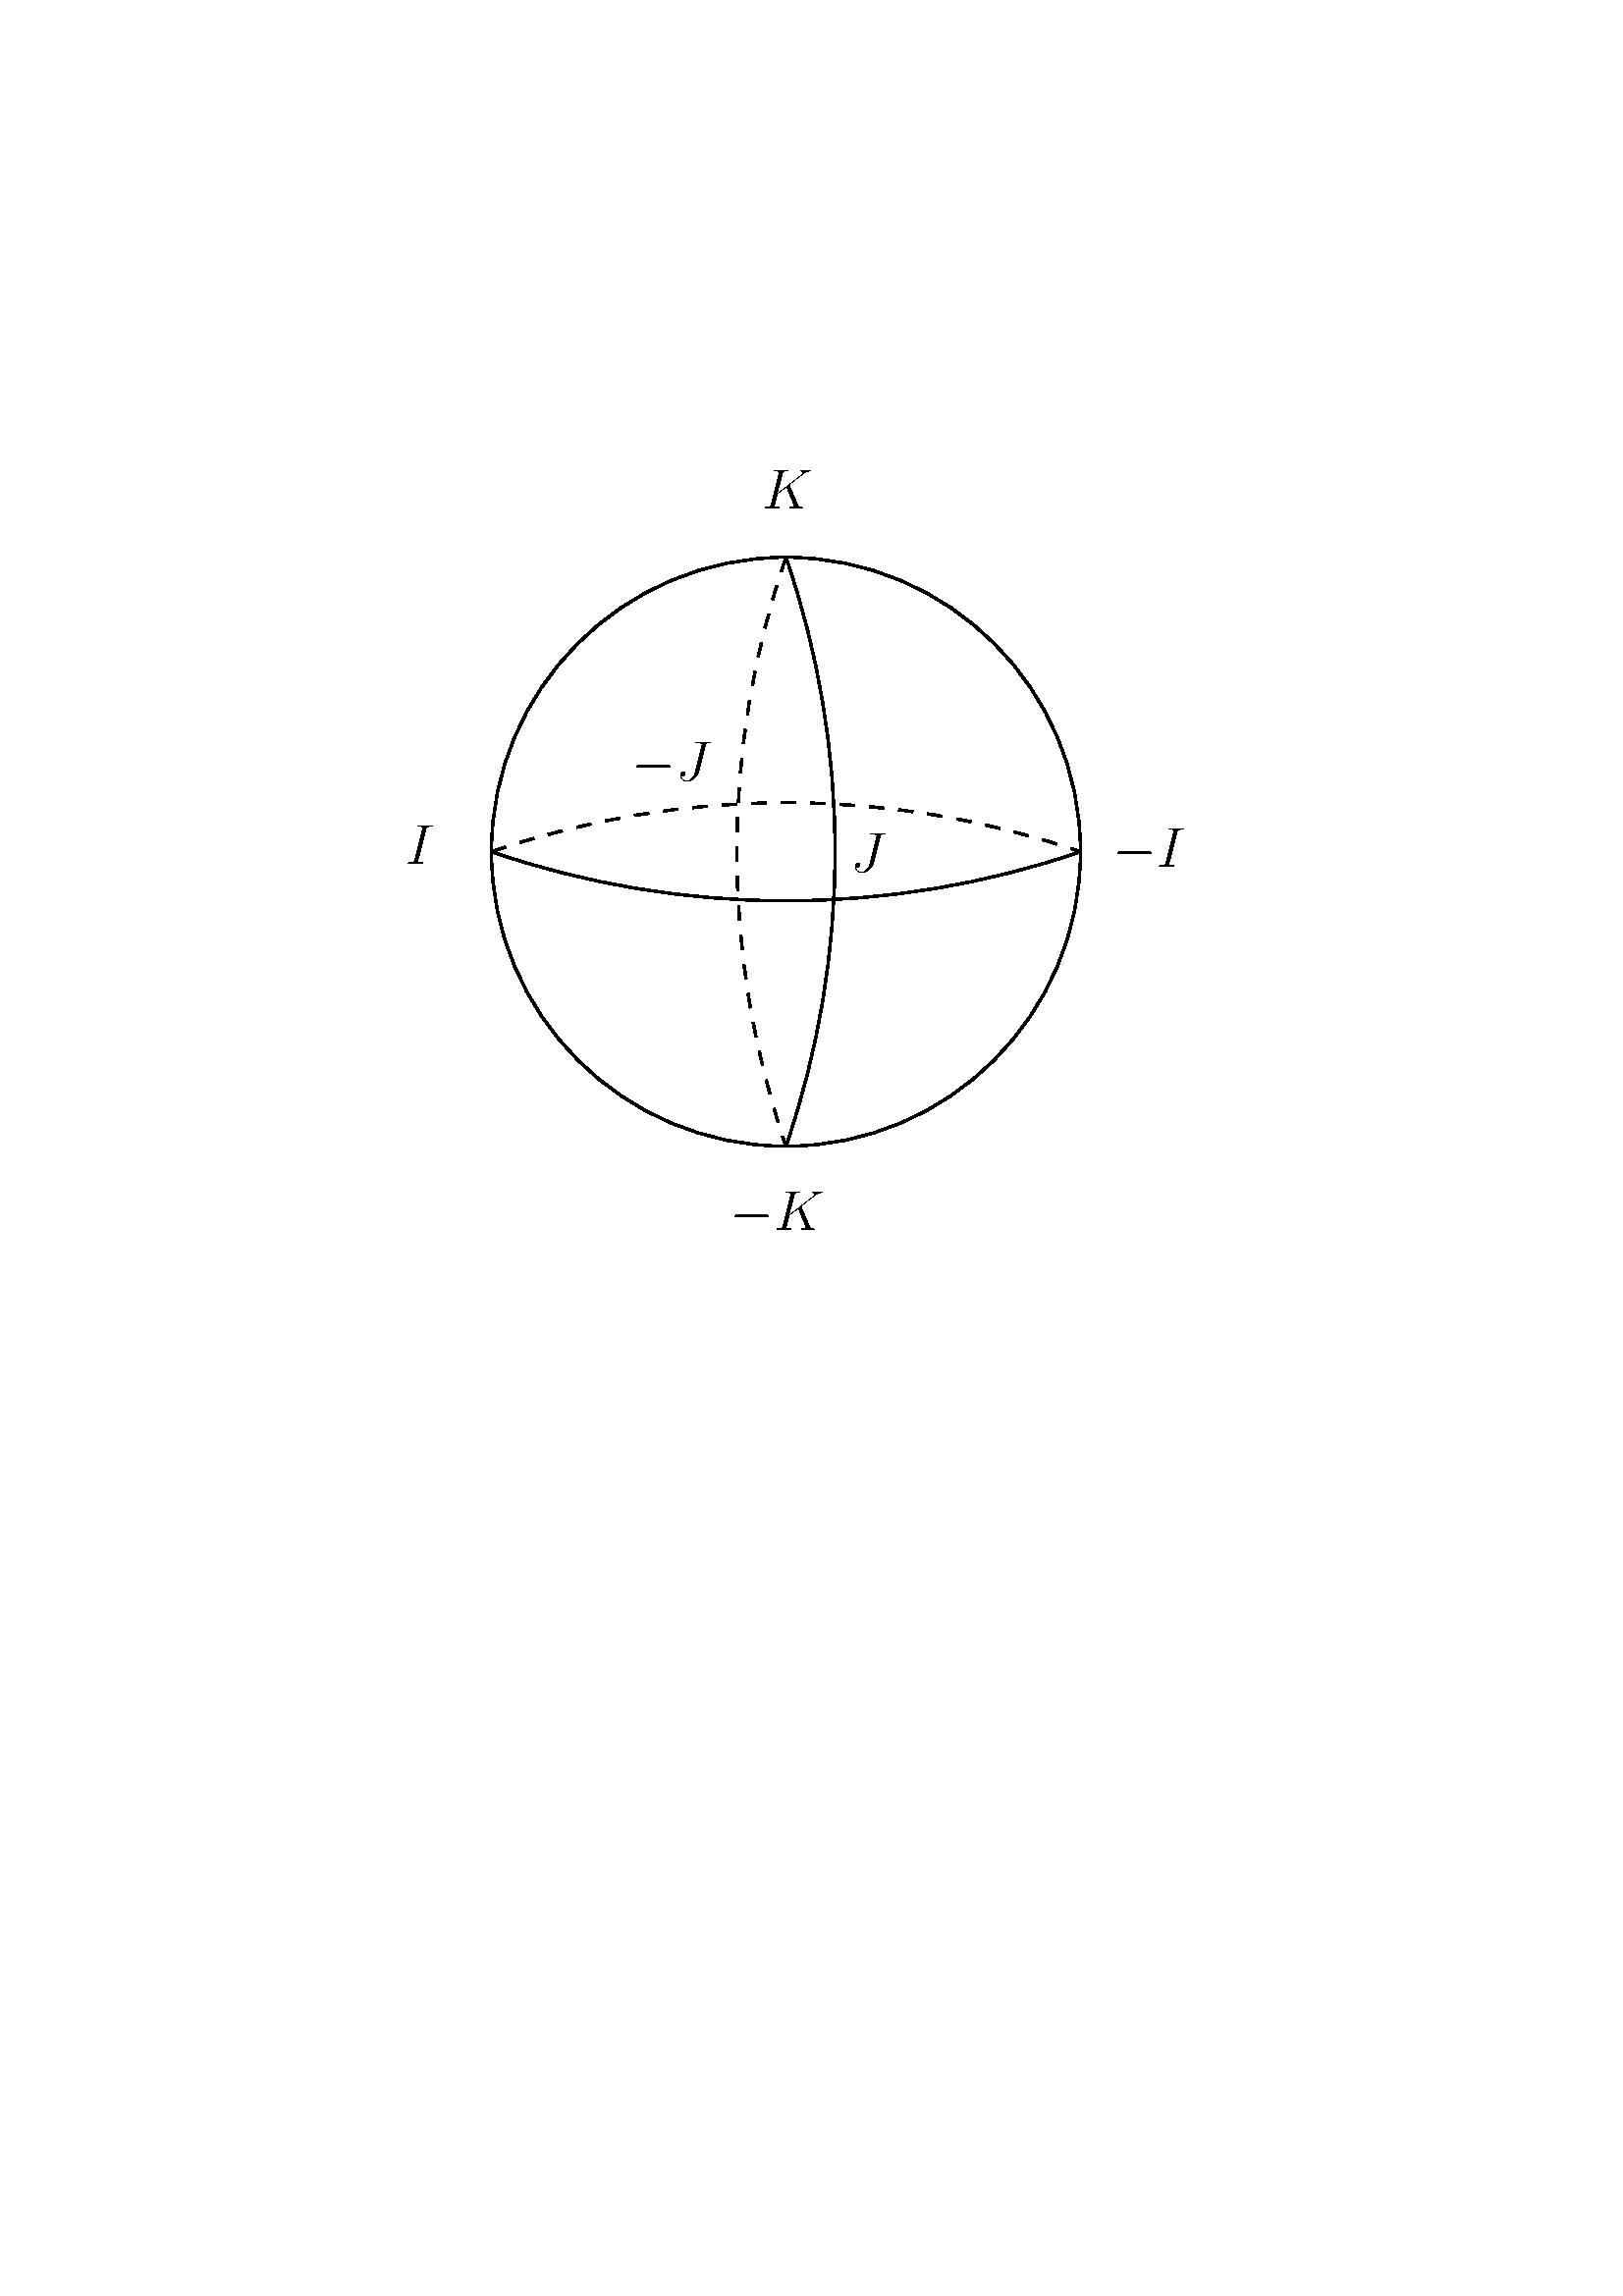
\includegraphics[width=0.75\linewidth]{figures/gla0-2.png}
\caption{ \medskip A family of complex structures on the hyper-Kahler manifold $\M_H$.（原文 Fig.~2）}
\label{fig:xunko}
\end{figure}
 A complex structure such as
$I, J,$ or $K$ is usually defined as a linear transformation of
the tangent space, but instead we will write down the transposed
matrices $I^t$, $J^t$, and $K^t$ acting on the cotangent space.
 We define $I^t$ by the formulas % 式 (4.3)
\setcounter{equation}{2}
\begin{equation}\label{eq:uttu}
\begin{aligned} I^t(\delta A_{\bar z} )& =
i\delta A_{\bar z} \\ I^t(\delta \phi_{z}) & = i\delta \phi_{ z}
\\ I^t(\delta A_{ z}) & = -i\delta A_{ z} \\ I^t(\delta
\phi_{\bar z}) & = -i\delta \phi_{\bar z}, \\\end{aligned}
\end{equation}
 which do ensure
$I^2=(I^t)^2=-1$. A translation-invariant complex structure on an
affine space $\EUW$ can also be characterized by saying which
linear functions on $\EUW$ are holomorphic.  For complex structure
$I$, the linear holomorphic functions are $A_{\bar z}$ and
$\phi_z$, evaluated at any point on $C$.

Similarly, we define a complex structure $J$ by
% 式 (4.4)
\setcounter{equation}{3}
\begin{equation}\label{eq:buttu}
\begin{aligned}J^t(\delta A_{\bar z}) & = -\delta \phi_{\bar
z}\\ J^t(\delta A_z) & = -\delta \phi_z \\  J^t(\delta\phi_{\bar
z}) &  = \delta A_{\bar z} \\ J^t(\delta \phi_{ z}) & = \delta
A_z.\\\end{aligned}
\end{equation}
  The linear holomorphic functions are $\CA_{\bar
z}=A_{\bar z}+i\phi_{\bar z}$ and $\CA_z=A_{z}+i\phi_z$, or more
succinctly $\CA=A+i\phi$.

Finally, we define complex structure $K$ by
% 式 (4.5)
\setcounter{equation}{4}
\begin{equation}\label{eq:bluttu}
\begin{aligned}K^t(\delta A_{\bar z} )& = -
i\delta\phi_{\bar z} \\ K^t(\delta \phi_{\bar z}) & = - i\delta
A_{\bar z} \\ K^t(\delta A_{ z} )& =  i\delta\phi_{ z} \\
K^t(\delta \phi_{ z}) & = i\delta A_{ z}. \\\end{aligned}
\end{equation}
 The linear
holomorphic functions are $A_{\bar z}-\phi_{\bar z}$ and
$A_z+\phi_z$.

These linear transformations of the cotangent space of $\EUW$ obey
$I^tJ^t=-J^tI^t=-K^t$, and cyclic permutations thereof. Taking the
transpose, we get the usual form of the quaternion relations
$IJ=-JI=K$, etc.

Beyond the quaternion relations, the definition of a hyper-Kahler
structure requires that the metric $ds^2$ should be of type
$(1,1)$ in each complex structure.  Equivalently, we want
$ds^2=I^t\otimes I^t(ds^2)=J^t\otimes J^t(ds^2)=K^t\otimes
K^t(ds^2).$ This can be readily verified.  Because $\EUW$ is an
affine space and our complex structures are linear, there is
nothing else to check; we have obtained a flat hyper-Kahler
structure on $\EUW.$

A hyper-Kahler manifold has (\xunko) a family of complex
structures parametrized by $\Bbb{CP}^1$, obtained by taking linear
combinations of $I,$ $J$, and $K$.  In the case at hand, we can
describe this family simply.  For any $w\in \Bbb{C}^*$, we
consider the complex structure $I_w$ in which $A_{\bar
z}-w\phi_{\bar z}$ and $A_z+w^{-1}\phi_z$ are holomorphic. Thus,
$w=-i$ corresponds to complex structure $J$, and $w=1$ corresponds
to $K$.  We extend the definition to include $w=0,\infty$ by
setting $I_0=I$, and $I_\infty=-I$ (here $-I$ is the complex
structure opposite to $I$, in which $A_z$ and $\phi_{\bar z}$ are
holomorphic), as these are the limits of $I_w$ for $w\to
0,\infty$. So we get the expected family of complex structures,
parametrized by a copy of $\Bbb{CP}^1$ that we will call
$\Bbb{CP}^1_h$ (see \zunko). An explicit formula for $I_w$ is
% 式 (4.6)
\setcounter{equation}{5}
\begin{equation}\label{eq:wyre}
I_w={1-\bar w w\over 1+\bar w w}I+{i(w-\bar w)\over
1+\bar w w}J+{w+\bar w\over 1+\bar w w}K.
\end{equation}
 Of course, this is of
the form $aI+bJ+cK$ with $a^2+b^2+c^2=1$.

\def\CU{{\cal U}}
We introduce a group $\CU_1\cong U(1)$ that acts on $\phi$ by
$\phi_z\to \lambda\phi_z$, $\phi_{\bar z}\to
\lambda^{-1}\phi_{\bar z}$, $|\lambda|=1$, while leaving $A$
fixed. $\CU_1$ preserves the hyper-Kahler metric and acts on
$\Bbb{CP}^1_h$ by % 式 (4.7)
\setcounter{equation}{6}
\begin{equation}\label{eq:zungo}
I_w\to I_{\lambda^{-1}w};
\end{equation}

 it leaves
fixed the two points $w=0,\infty$.  We explain at the end of
section 第~\ref{sec:complexstr}~节\ in what sense the action of $\CU_1$ extends
to an action of its complexification $\CU\cong \Bbb{C}^*$.

Most of the complex structures on $\EUW$ in this family depend on
the complex structure of $C$.  The exceptions are $J$, which can
be characterized as the complex structure in which $\CA=A+i\phi$
is holomorphic, and $-J$, in which $\bar\CA=A-i\phi$ is
holomorphic.  The other complex structures on $ \EUW$ treat
differently the $z$ and $\bar z$ components of $A$ and $\phi$, a
distinction that depends on the complex structure of $C$.

Does the symmetry group ${\cal U}_1$  come from a symmetry of
four-dimensional Yang-Mills theory?  The answer to this question
is a little subtle.  The twisted ${\EUN}=4$ super Yang-Mills
theory compactified on $C$ does have the symmetry group $\CU_1$.
It acts by rotation of the $\phi_2-\phi_3$ plane; this is a
subgroup of $SU(4)_{\cal R}$ that is unbroken in this particular
compactification. However, this does not give a symmetry of the
underlying family of four-dimensional TQFT's, because it does not
preserve the family of supersymmetry generators
$\epsilon=u\epsilon_\ell+v\epsilon_\rr$ (it maps this family to a
larger family, whose interpretation we discuss in section
第~\ref{sec:twistedtft}~节, of supersymmetries that lack the full $Spin'(4)$
symmetry).

But the element $-1\in {\cal U}_1$ does arise from a symmetry of
the four-dimensional TQFT. This element acts on $\MH$ just like
the central element ${\EUI}\in SU(4)_{\cal R}$, which we
introduced in section 第~\ref{sec:reviewsd}~节. Indeed, ${\EUI}$ acts as $i$ in
the ${\bf 4}$ of $SU(4)_{{\cal R}}$, so it acts as $-1$ on ${\bf
6}=\wedge^2{\bf 4}$, which is the representation that contains
$\phi$.  (Note that ${\EUI}$ also reverses the sign of untwisted
scalars.) The transformation $\phi\to-\phi$ is holomorphic in
complex structure $I$, but antiholomorphic in structures $J$ and
$K$.  The obvious component of the fixed point set of this
transformation is defined by $\phi=0$ (giving, as we discuss
later, an embedding of $\M$, the moduli space of stable bundles,
in $\MH$).  There also are \cite{ref20}\ other components of the fixed
point set in which $\phi$ is gauge-equivalent to $-\phi$.

\par\medskip{\it Symplectic Structures}

The three symplectic structures associated with the hyper-Kahler
structure on $\EUW$ can be defined as $\omega_I = I^t\otimes
1(ds^2)$, and similarly  $\omega_J=J^t\otimes 1(ds^2) $ and
$\omega_K=K^t\otimes 1(ds^2)$. We get % 式 (4.8)
\setcounter{equation}{7}
\begin{equation}\label{eq:tomog}
\begin{aligned}\omega_I
& = -{i\over 2\pi}\int_C|d^2z|\,\Tr\left(\delta A_{\bar z}\wedge
\delta A_z-\delta \phi_{\bar z}\wedge \delta\phi_z\right)\\
&=-{1\over 4\pi}\int_C\,\Tr\left(\delta A\wedge \delta A
-\delta\phi\wedge\delta \phi\right) \\
                      \omega_J & ={1\over 2\pi}\int_C |d^2z|\,\Tr\left(
                      \delta\phi_{\bar z}\wedge \delta A_z+\delta\phi_z\wedge
                      \delta A_{\bar z} \right)\\
                      \omega_K & =
                      {i\over 2\pi}\int_C|d^2z|\,\Tr\left(\delta\phi_{\bar z}
                      \wedge\delta A_z-\delta\phi_z\wedge\delta A_{\bar z}\right)\\
                      & = {1\over 2\pi}\int_C \,\Tr\,\delta\phi
                      \wedge\delta A.\\\end{aligned}
\end{equation}

Here, $\omega_J$ depends on the complex structure of $C$, while
$\omega_I$ and $\omega_K$ do not.

Moreover, $\omega_I$ is of type $(1,1)$ with respect to complex
structure $I$, and similarly for $\omega_J$ and $\omega_K$.  We
also define $\Omega_I=\omega_J+i\omega_K$, along with cyclic
permutations $\Omega_J=\omega_K+i\omega_I$,
$\Omega_K=\omega_I+i\omega_J$:
 % 式 (4.9)
\setcounter{equation}{8}
\begin{equation}\label{eq:ninto}
\begin{aligned}\Omega_I & =
{1\over \pi}\int_C|d^2z|\,\Tr\,\delta\phi_z\wedge \delta A_{\bar
z} \\
        \Omega_J & =-{i\over 4\pi}\int_C\,\Tr\,\delta \CA\wedge\delta \CA          \\
        \Omega_K & = -{i\over 2\pi}\int_C |d^2z|\,\Tr\,\left( \delta A_{\bar z}\wedge
\delta A_z-\delta \phi_{\bar z}\wedge \delta\phi_z -
\delta\phi_{\bar z}\wedge \delta A_z-\delta\phi_z\wedge
                      \delta A_{\bar z}\right).\\\end{aligned}
\end{equation}

$\Omega_I$ is of type $(2,0)$ in complex structure $I$, and
similarly $\Omega_J$ and $\Omega_K$ are of type $(2,0)$ in their
respective complex structures. $\Omega_I$ and $\Omega_K$ depend on
the complex structure of $C$, but $\Omega_J$ does not.

The closed two-forms $\omega_J$ and $\omega_K$ are actually exact.
Indeed, we can write very explicitly $\omega_J=\delta\lambda_J$
with $\lambda_J={1\over 2\pi}\int_C |d^2z|\,\Tr\,\left(\phi_{\bar
z}\delta A_z+\phi_z\delta A_{\bar z}\right)$. $\lambda_J$ is
gauge-invariant, because $\phi$ and $\delta A$ (unlike $A$ itself)
both transform in the adjoint representation of $G$.  Similarly
$\omega_K=\delta\lambda_K$ with $\lambda_K={1\over
2\pi}\int_C\,\Tr\,\phi\wedge \delta A$. Among other things, this
means that a topologically trivial line bundle over $\MH$ can be
endowed with a  connection whose  curvature is any desired linear
combination of $\omega_J$ and $\omega_K$.  One simply picks the
connection to be a suitable linear combination of $\lambda_J$ and
$\lambda_K$.

 
On the other hand, $\omega_I$ is topologically non-trivial.  To
write $\omega_I=\delta\lambda_I$ along the above lines, one would
need in $\lambda_I$ a term proportional to $\int \Tr \,A\wedge
\delta A$, but this is not gauge-invariant because of the
inhomogeneous transformation of $A$ under gauge transformations.
However, we can write $\omega_I=\omega_I'+\delta\lambda_I$, where
$\lambda_I=(1/4\pi)\int_C\Tr\,\phi\wedge\delta\phi$ and
% 式 (4.10)
\setcounter{equation}{9}
\begin{equation}\label{eq:frox}
\omega_I'=-{1\over 4\pi}\int_C\Tr\,\delta A\wedge\delta
A.
\end{equation}
 So $\omega_I$ and $\omega_I'$ are cohomologous, and in
particular the cohomology class of $\omega_I$ is a pullback from
the subspace with $\phi=0$.  For simply-connected $G$, the Picard
group of line bundles over $\M$ is $\Bbb{Z}$, generated by a line
bundle ${{\frak L}}$  whose first Chern class is represented in de
Rham cohomology by $\omega_I'/2\pi$.  We will loosely call
${{\frak L}}$ the determinant line bundle, since for classical $G$
it can be defined \cite{ref60}\ as the determinant of a $\bar\partial$
operator.\footnote{For $G=SU(N)$, if $E\to C$ is a holomorphic vector
bundle of rank $N$, the fiber ${\frak L}_E$ at $E$ of the
determinant line bundle $\frak L$ is ${\frak
L}_E=\det\,H^0(C,E)^{-1}\otimes \det\, H^1(C,E)$, where $\det\,V$
denotes the highest exterior power of a vector space $V$.  The
line bundle $\frak L\to \M$ so defined is ample.  Some authors
write ${\frak L}^{-1}$ for what we call $\frak L$.}

\par\medskip{\it Hitchin Moduli Space as a Hyper-Kahler Quotient}

We now consider the group of gauge transformations acting on
$\EUW$ in an obvious way. It manifestly preserves the metric
\eqref{eq:igob}\ and the three symplectic structures \eqref{eq:tomog} . A short
computation shows that the Hitchin equations \eqref{eq:zongo}\ are
equivalent to the vanishing of the three moment maps corresponding
to the symplectic structures \eqref{eq:tomog}. Explicitly, let $\epsilon$
generate an infinitesimal gauge transformation  (thus, $\epsilon$
is a zero-form with values in ${\rm ad}(E)$), and let
$V(\epsilon)$ be the corresponding vector field on $\EUW$, which
acts by $\delta A=-D\epsilon$, $\delta\phi=[\epsilon,\phi]$. Then
the moment map $\mu$ for symplectic structure $\omega$ is found by
solving the condition $\iota_{V(\epsilon)}\omega=\delta\mu$ (here
$\iota_{V(\epsilon)}$ is the operator of contraction with
$V(\epsilon)$). Taking $\omega$ to be $\omega_I$, $\omega_J$, or
$\omega_K$, the corresponding moment maps turn out to be
% 式 (4.11)
\setcounter{equation}{10}
\begin{equation}\label{eq:joget}
\begin{aligned}\mu_I & =-{1\over
2\pi}\int_C\,\Tr\,\epsilon(F-\phi\wedge \phi),\\ \mu_J &
=-{1\over 2\pi}\int_C|d^2z|\,\Tr\,\epsilon\left(D_z\phi_{\bar
z}+D_{\bar z}\phi_z\right), \\ \mu_K& = -{i\over
2\pi}\int_C|d^2z|\,\Tr\,\epsilon\left(D_z\phi_{\bar z}-D_{\bar
z}\phi_z\right).\\\end{aligned}
\end{equation}
 In general, if $X$ is a hyper-Kahler
manifold on which a Lie group $H$ acts with moment maps
$\vec\mu=(\mu_I,\mu_J,\mu_K)$, then the quotient by $H$ of the
solution set of the equations $\vec\mu=0$ is a hyper-Kahler
manifold \cite{ref61}, called the hyper-Kahler
quotient $X/\negthinspace/\negthinspace/H$ of $X$ by $H$. So in
particular $\M_H$ is the hyper-Kahler quotient of the
infinite-dimensional space ${\EUW}$ by the group of gauge
transformations, and is a hyper-Kahler manifold.

It is possible to give a more ``physical'' explanation of why the
target of the sigma-model is the hyper-Kahler quotient of $\EUW$.
In general, in a two-dimensional gauge theory with $(4,4)$
supersymmetry and gauge group $H$, the hypermultiplets parametrize
a hyper-Kahler manifold $X$, and the low energy physics (assuming
for simplicity that $H$ acts freely on $X$) is a sigma-model with
target the hyper-Kahler quotient
$X/\negthinspace/\negthinspace/H$. (This is the context in which
the hyper-Kahler quotient construction was originally discovered
\cite{ref61}.) In the present example, compactification of the
twisted topological gauge theory in four dimensions give in two
dimensions a theory with $(4,4)$ supersymmetry.  (The twisting and
compactification preserve eight of the original sixteen
supersymmetries, of which four have one two-dimensional chirality
and four have the other.) The gauge group of this two-dimensional
theory is the group ${\cal G}$ of maps of $C$ to $G$, and the
hypermultiplets parametrize $\EUW$. This is precisely the setup
that leads to $\MH$ as a hyper-Kahler quotient.  So the low energy
physics is a sigma-model with target the hyper-Kahler quotient of
$\EUW$.

\par\medskip{\it More Precise Account Of Dimensional
Reduction}

We can now be more precise about the dimensional reduction from
twisted four-dimensional super  Yang-Mills theory to the
sigma-model with target $\MH$.  Such a sigma-model has a metric
and a $B$-field.  We want to determine what they are.

We consider four-dimensional super Yang-Mills on $M=\Sigma\times
C$, where the radius of $\Sigma $ is much greater than the radius
of $C$.  The kinetic energy of the gauge fields is
% 式 (4.12)
\setcounter{equation}{11}
\begin{equation}\label{eq:kinen}
{{\cmmib I}}_{kin}=-{1\over 2e^2}\int_{\Sigma\times C}
|d^2y|\,|d^2z|\,\Tr\,F_{\mu\nu}F^{\mu\nu},
\end{equation}
 where $|d^2y|$ and
$|d^2z|$ are the Riemannian measures on $\Sigma$ and $C$,
respectively. This has contributions of type $(p,q)$, $p+q=2$,
where $p$ is the number of indices $\mu,\,\nu$ that are tangent to
$\Sigma$ and $q$ is the number tangent to $C$. It is useful to
write the gauge field on $\Sigma\times C$ as $A=A_\Sigma+A_C$,
where $A_\Sigma$ is tangent to $\Sigma$ and $A_C$ is tangent to
$C$.

The terms of type $(0,2)$ are part of the potential energy for
$A_C$ that causes the theory to be localized on slowly varying
maps  $\Phi:\Sigma\to \MH$. The terms of type $(2,0)$ give a
kinetic energy for $A_\Sigma$, which away from singularities of
$\MH$ is massive, because the gauge group is completely broken,
and can be integrated out in the infrared (as we describe
explicitly in section 第~\ref{sec:wilbranes}~节).

The kinetic energy for the sigma-model comes from the terms of
type $(1,1)$.  These terms are % 式 (4.13)
\setcounter{equation}{12}
\begin{equation}\label{eq:binen}
-{1\over e^2}\int
|d^2y|\,|d^2z|\,\sum_{\mu=0,1}\sum_{\nu=2,3}\,\Tr\,F_{\mu\nu}F^{\mu\nu}.
\end{equation}

We want to compare this to a general sigma-model of maps
$\Phi:\Sigma\to X$, where the target space $X$ has metric
$ds^2_X=g_{IJ}(X)\,dX^I\,dX^J$ in terms of local coordinates
$X^I$.  The kinetic energy of the sigma-model is then
% 式 (4.14)
\setcounter{equation}{13}
\begin{equation}\label{eq:zinen}
\int |d^2y|\, g_{IJ}\sum_{\mu=0,1}\partial_\mu
X^I\partial^\mu X^J.
\end{equation}
 In comparing \eqref{eq:binen}\ and \eqref{eq:zinen}, the role of
the $X^I$ is played by $A_C$, and $F_{ij}$ corresponds to
$\partial_i X^I$.  If we compare \eqref{eq:binen}\ and \eqref{eq:zinen}\ to our
original definition \eqref{eq:igob}\ of the hyper-Kahler metric $ds^2$ on
${\EUW}$ (which induces   on the hyper-Kahler quotient $\MH$ a
metric that we also call $ds^2$), we see that the metric $ds^2_g$
that is induced by the four-dimensional gauge theory is related to
$ds^2$ by % 式 (4.15)
\setcounter{equation}{14}
\begin{equation}\label{eq:inog}
ds^2_g={4\pi\over e^2}\,ds^2=({\rm
Im}\,\tau)\,ds^2.
\end{equation}

We similarly want to reduce the $\theta$ term of the gauge theory,
which in Euclidean signature is % 式 (4.16)
\setcounter{equation}{15}
\begin{equation}\label{eq:bloko}
{\cmmib
I}_\theta={i\theta\over 8\pi^2}\int_{\Sigma\times C}\,\Tr\,
F\wedge F.
\end{equation}
 Again, we evaluate this coupling for a gauge field
that represents a slowly varying map to $\MH$.  Because of the
topological invariance of ${{\cmmib I}}_\theta$, in evaluating
\eqref{eq:bloko}\ we can deform to a situation in which the restriction of
$F$ to $C$ vanishes (that is, $F_{23}=0$).  The deformation to
$F|_C=0$ can be achieved via a complex gauge transformation or
using Hitchin's second fibration $\MH\to\M$ (these are both
notions that we explain later).  Given this, in evaluating
${\cmmib I}_\theta$, we can replace $F={1\over
2}\sum_{\mu,\nu=0}^3dx^\mu\wedge dx^\nu \,F_{\mu\nu}$ by
$F^{1,1}=\sum_{\mu=0,1}\sum_{\nu=2,3}dx^\mu\wedge dx^\nu
\,F_{\mu\nu}$. In the sigma-model limit, $F^{1,1}$ corresponds to
$\delta A_C=\sum_{\mu=0,1}dx^\mu \,D_\mu A_C$, and ${\cmmib
I}_\theta$ reduces to\footnote{A minus sign enters because in defining
$\omega_I'$, $\delta$, the exterior derivative on the space of
connections $A_C$, is taken to commute with a one-form on $C$ such
as $dx^ j$, $j=2,3$, which does not depend on $A_C$. For
differential forms on $\Sigma\times C$, in terms of which ${\cmmib
I}_\theta$ is defined, they would anticommute.}
% 式 (4.17)
\setcounter{equation}{16}
\begin{equation}\label{eq:ino}
-{i\theta\over 8\pi^2}\int_\Sigma \int_C \Tr\,\delta
A_C\wedge \delta A_C.
\end{equation}

Comparing to the definition \eqref{eq:frox}\ of $\omega_I'$, we see that
this is equivalent to % 式 (4.18)
\setcounter{equation}{17}
\begin{equation}\label{eq:zinok}
{i\theta\over
2\pi}\int_\Sigma\Phi^*(\omega'_{I})={i\theta\over 2\pi}\int_\Sigma
\Phi^*(\omega_I),
\end{equation}
 where the last step uses the fact that
$\omega_{I}-\omega'_{I}$ is exact.  In the general sigma-model,
the $B$-field is a closed two-form on the target space $X$; it
appears in the action via a term $-i\int_\Sigma\,\Phi^*(B)$. So
the $B$-field of the effective low energy sigma-model is
% 式 (4.19)
\setcounter{equation}{18}
\begin{equation}\label{eq:palooka}
B=-{\theta\over 2\pi}\omega_I=-({\rm
Re}\,\tau)\,\omega_I.
\end{equation}

We can describe this more conceptually.  For simply-connected $G$,
the instanton number $(1/8\pi^2)\int_M \Tr\,F\wedge F$ is
integer-valued for any four-manifold $M$.  In addition, for
simply-connected $G$, $\MH$ is simply-connected, and hence
$H^2(\MH,\Bbb{Z})=\pi_2(\MH)$.  The form $\omega_I$ has been
normalized so that $\omega_I/2\pi$ is the image in de Rham
cohomology of a generator of $H^2(\MH,\Bbb{Z})$. These facts imply
that for any $\Sigma$ and $C$, there is a map $\Phi:\Sigma\to \MH$
with $\int_\Sigma\Phi^*(\omega_I/2\pi)=1$ (and this is the smallest
achievable value).  Such a map corresponds to a gauge field on
$M=\Sigma\times C$ that has instanton number $\pm 1$ depending on
one's conventions.\footnote{In the physics literature, instantons in
four dimensions are generally taken to be selfdual gauge fields,
obeying $F^-=0$, and in the math literature, they are generally
taken to be anti-selfdual, obeying $F^+=0$.  If an instanton in
the sigma model is understood as a holomorphic map to $\MH$, and
the usual physics convention is followed in four dimensions, then
a sigma model field of instanton number 1 comes from a gauge
theory instanton of instanton number $-1$.  The usual math
convention  avoids this minus sign.} More briefly, the theta
angles are the same in two and four dimensions because the
instantons are the same. If $G$ is not simply-connected, things
are a little more complicated; the instanton number is not always
an integer, and there are corresponding complications on the
sigma-model side.
